\section{Efficiency Beyond Quantisation}

\begin{frame}{}
    \LARGE Research Frontiers: \textbf{Efficiency Beyond Quantisation}

    \vspace{1em}
    \normalsize The weights are already 4-bit. Where does the next speedup come from?
\end{frame}

\subsection{Speculative Decoding Without a Draft Model}

\begin{frame}{Speculative Decoding in One Slide}
    \begin{itemize}\itemsep0.5em
        \item \textbf{The idea.} A small \emph{draft} model proposes $K$ tokens one by one. The large \emph{target} model then checks all $K$ in a single forward pass, which costs about the same as generating one token.
        \item \textbf{The rule.} Draft token $\tilde x$ is kept with probability $\min\!\big(1,\, q(\tilde x)/p(\tilde x)\big)$, where $p$ is the draft's distribution and $q$ the target's. At the first rejection, that position is resampled from the normalised positive part of $q-p$ and the rest of the draft is discarded.
        \item \textbf{The guarantee.} The output distribution is exactly the target model's. Speed comes only from accepting several tokens per target pass.
        \item \textbf{The original result.} 2 to 3x faster decoding with no change in output quality.
    \end{itemize}
    \vspace{0.3em}
    \takeaway{The methods on the next slides remove the separate draft model (Medusa, EAGLE) or make the verification cheaper. The acceptance rule stays the same.}
    \src{Leviathan, Kalman, Matias, ``Fast Inference from Transformers via Speculative Decoding,'' \href{https://arxiv.org/abs/2211.17192}{arXiv:2211.17192}. Chen et al., ``Accelerating Large Language Model Decoding with Speculative Sampling,'' \href{https://arxiv.org/abs/2302.01318}{arXiv:2302.01318}.}
\end{frame}

\begin{frame}{Speculative Decoding Pays Off Only at Small Batch}
    \begin{itemize}\itemsep0.2em
        \item \textbf{Why it works.} Generating one token per sequence reads all the weights for one small matrix-vector product, so the GPU waits on memory and its compute sits idle. Verifying several drafted tokens in one pass uses that idle compute for free.
        \item \textbf{Why it stops working.} With many sequences in the batch, the compute is no longer idle. Verifying draft tokens now competes with real work, and the gain shrinks or turns into a loss.
    \end{itemize}
    \vspace{0.2em}
    \begin{center}
    \small
    \begin{adjustbox}{max width=\linewidth}\begin{tabular}{lccc}
        \toprule
        \textbf{Speed relative to plain decoding} & \textbf{batch 2} & \textbf{batch 16} & \textbf{batch 64} \\
        \midrule
        EAGLE-3 & 1.81x faster & 1.48x faster & 1.38x faster \\
        EAGLE-2 & 1.40x faster & \multicolumn{2}{c}{slower than plain decoding from batch 24 (0.88x to 0.99x)} \\
        \bottomrule
    \end{tabular}\end{adjustbox}

    {\scriptsize LLaMA-3.1-8B served with SGLang on one H100.}
    \end{center}
    \takeaway{Speculative decoding is a \textbf{low-batch latency} tool. Under heavy load, vLLM measured 1.4x to 1.8x \emph{slowdowns}.}
    \src{Liang, Stanford CS336 Lecture 10 (2025). Li et al., ``EAGLE-3,'' \href{https://arxiv.org/abs/2503.01840}{arXiv:2503.01840}, Table 3. vLLM Team, ``How Speculative Decoding Boosts vLLM Performance by up to 2.8x'' (Oct 2024).}
\end{frame}

\begin{frame}{Medusa: Let the Model Draft for Itself}
    \begin{columns}[T,onlytextwidth]
        \column{0.56\textwidth}
        \begin{itemize}\itemsep0.4em
            \item \textbf{Problem:} a separate draft model must be found, aligned and served.
            \item \textbf{Idea:} add $K$ small heads on the last hidden state. Head $k$ predicts the token $k+1$ steps ahead:
            \[
                p_t^{(k)} = \mathrm{softmax}\big(W_2^{(k)}\,(\mathrm{SiLU}(W_1^{(k)} h_t) + h_t)\big)
            \]
            \item \textbf{Medusa-1:} heads on a frozen backbone, over 2.2x. \textbf{Medusa-2:} joint training, 2.3 to 3.6x.
            \item Each step costs 1.18 to 1.27x more, so
            $\text{speedup} = \text{tokens per step} \,/\, \text{overhead}$.
        \end{itemize}
        \column{0.42\textwidth}
        \centering
        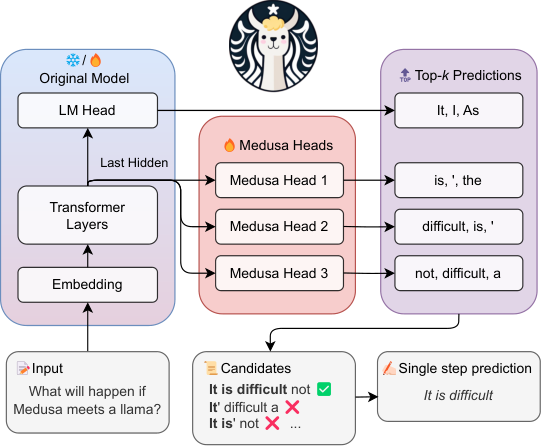
\includegraphics[width=\linewidth,height=0.6\textheight,keepaspectratio]{images/research-frontiers/medusa_fig1_architecture.png}
    \end{columns}
    \vspace{0.2em}
    \src{Cai, Li, Geng, Peng, Lee, Chen, Dao, ``Medusa: Simple LLM Inference Acceleration Framework with Multiple Decoding Heads,'' \href{https://arxiv.org/abs/2401.10774}{arXiv:2401.10774}, Figure 1 and Table 1.}
\end{frame}

\begin{frame}{Verifying a Whole Tree in One Forward Pass}
    \begin{columns}[T,onlytextwidth]
        \column{0.5\textwidth}
        \centering
        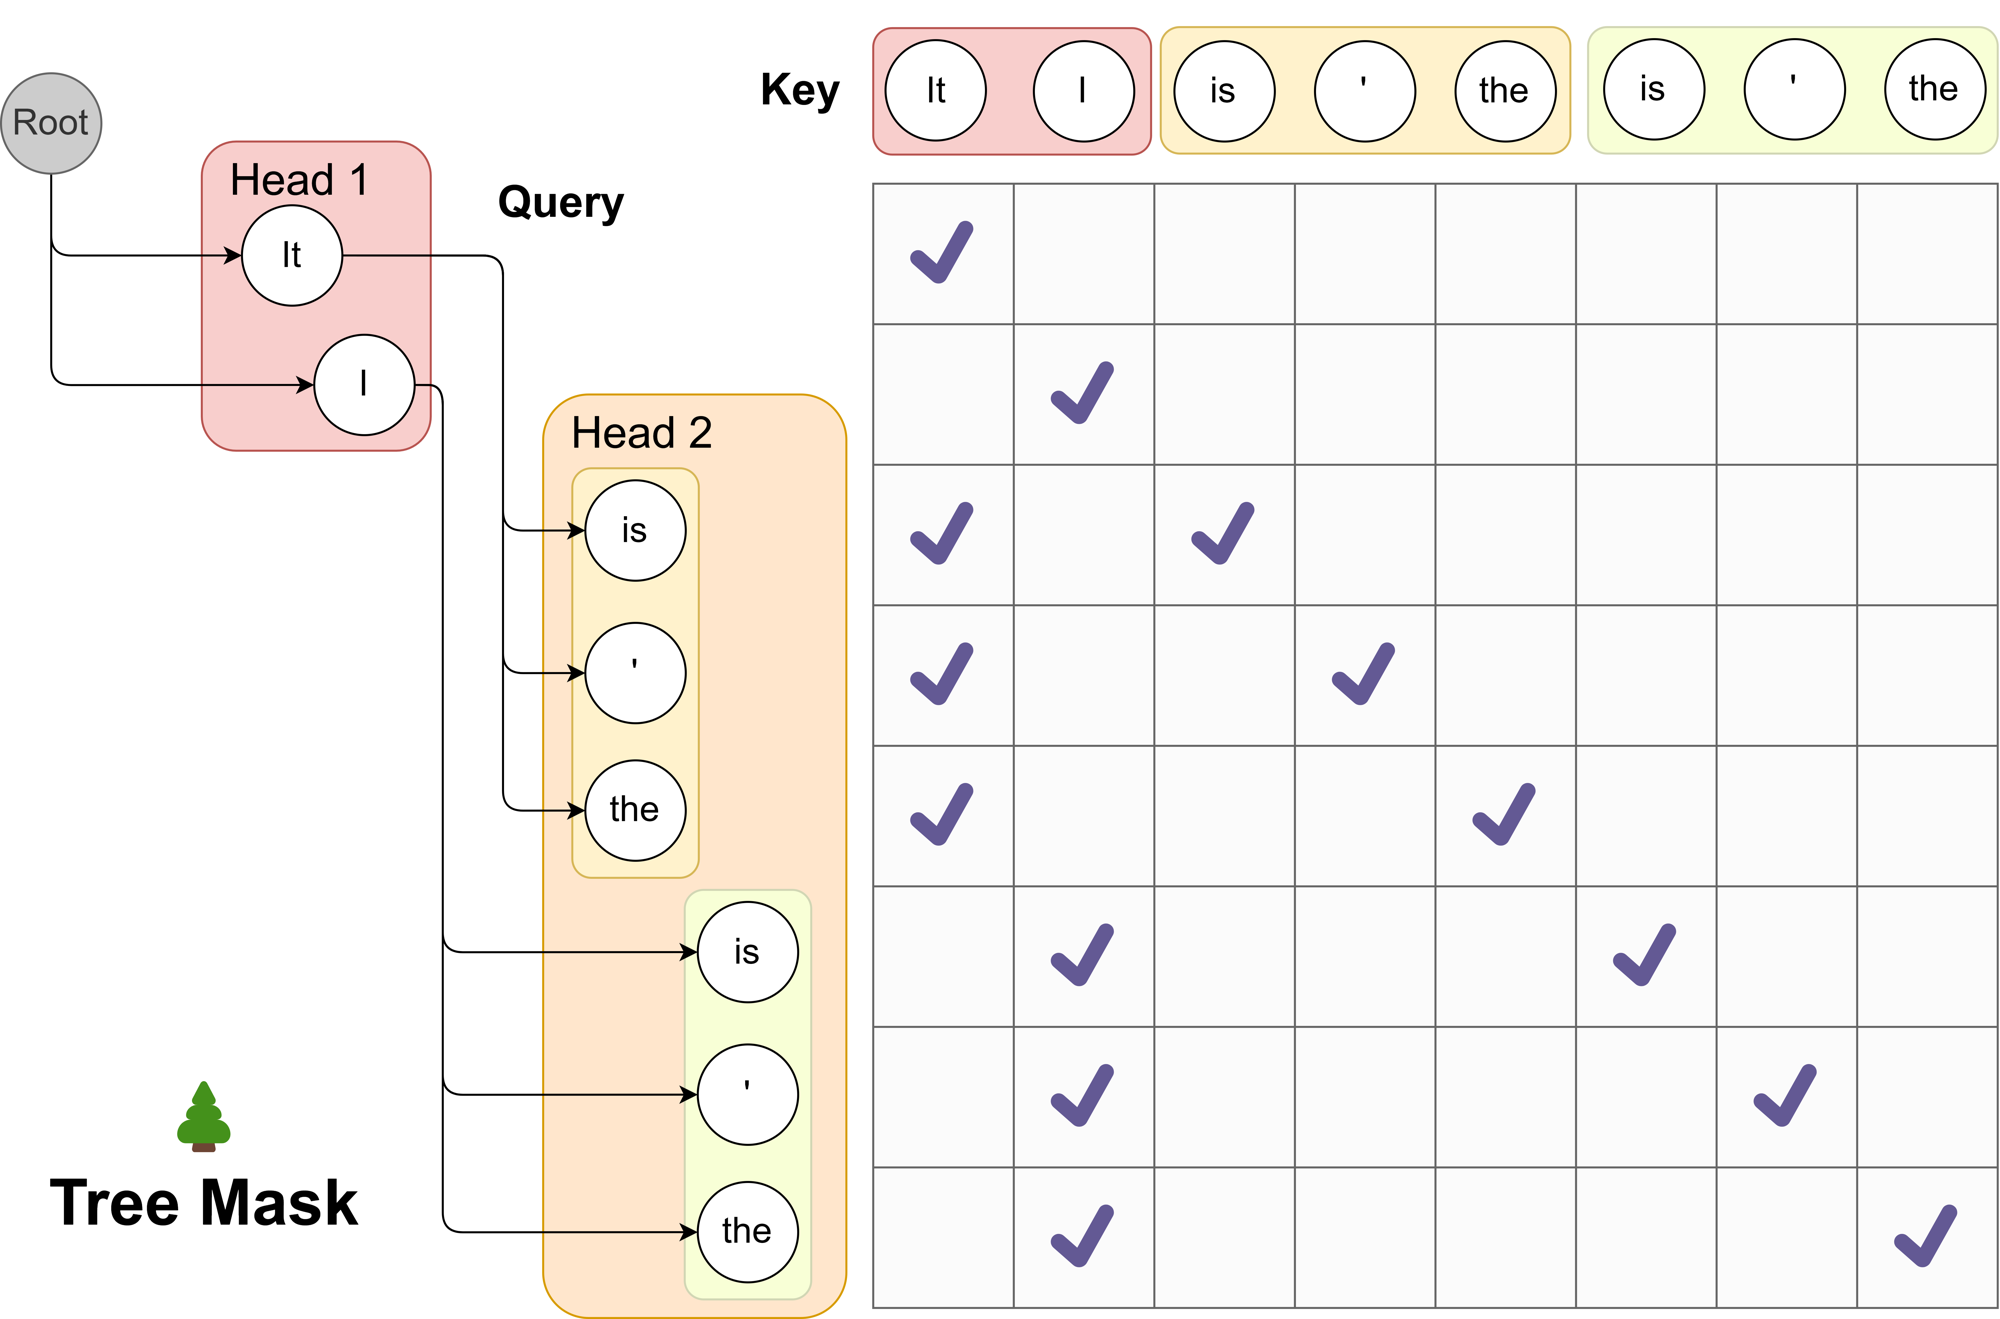
\includegraphics[width=\linewidth,height=0.58\textheight,keepaspectratio]{images/research-frontiers/medusa_fig2_tree_attention.png}
        \column{0.48\textwidth}
        \begin{itemize}\itemsep0.45em
            \item The top guesses of each head combine into a \textbf{tree of candidates}.
            \item A \textbf{tree attention mask} lets each candidate see only its ancestors. One pass scores every branch.
            \item Bigger is not better: a sparse 64-node tree beats a dense 256-node one.
            \item \textbf{Hydra} lets each head see the tokens drafted before it. Up to 1.31x over Medusa.
            \item \textbf{Lossy or lossless?} Medusa's \emph{typical acceptance} changes the output distribution. Standard verification does not.
        \end{itemize}
    \end{columns}
    \vspace{0.2em}
    \src{Cai et al., \href{https://arxiv.org/abs/2401.10774}{arXiv:2401.10774}, Figures 2 and 4. Ankner et al., ``Hydra: Sequentially-Dependent Draft Heads for Medusa Decoding,'' \href{https://arxiv.org/abs/2402.05109}{arXiv:2402.05109}.}
\end{frame}

\begin{frame}{EAGLE: Draft in Feature Space, Then Train as You Test}
    \begin{columns}[T,onlytextwidth]
        \column{0.6\textwidth}
        \begin{itemize}\itemsep0.35em
            \item \textbf{EAGLE (2024).} A one-layer drafter autoregresses over the target's \emph{hidden features}, not its tokens.
            \item \textbf{EAGLE-2.} The drafter's confidence predicts acceptance, so the tree grows where acceptance is likely.
            \item \textbf{EAGLE-3 (2025).} Predict tokens directly, and feed the drafter \emph{its own outputs} during training.
        \end{itemize}
        \begin{center}
        \small
        \footnotesize\setlength{\tabcolsep}{4pt}\begin{adjustbox}{max width=\linewidth}\begin{tabular}{lcc}
            \toprule
            \textbf{Vicuna-13B, MT-bench} & \textbf{Speedup} & \textbf{Tokens per step} \\
            \midrule
            Vanilla speculative sampling & 1.93x & 2.27 \\
            EAGLE-2 & 4.26x & 4.83 \\
            \rowcolor{KAUSTcyan!12} EAGLE-3 & 5.58x & 6.65 \\
            \bottomrule
        \end{tabular}\end{adjustbox}
        \end{center}
        \column{0.38\textwidth}
        \centering
        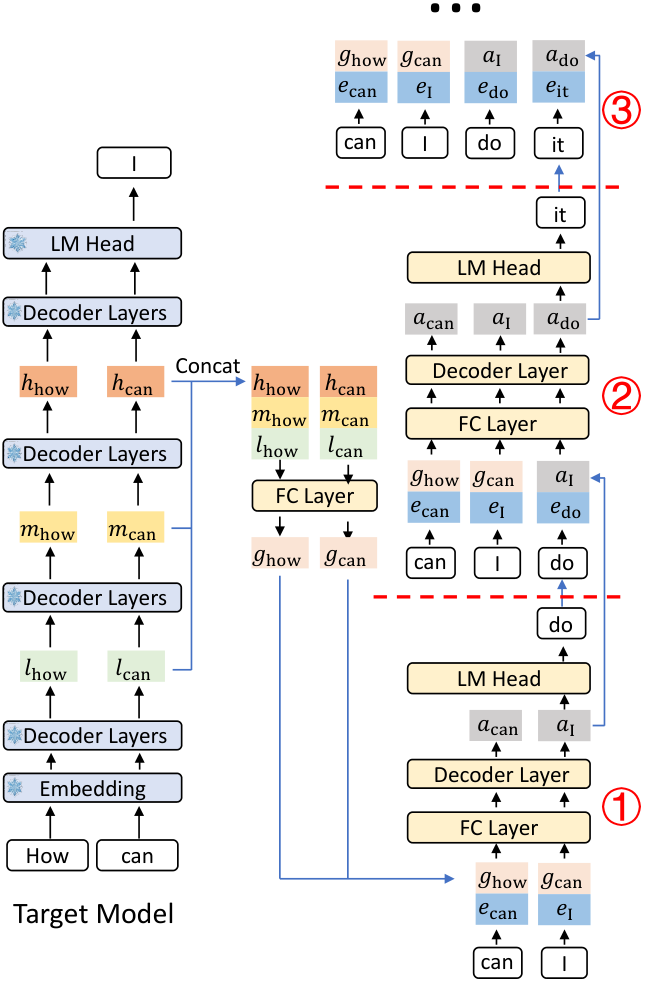
\includegraphics[width=\linewidth,height=0.64\textheight,keepaspectratio]{images/research-frontiers/eagle3_method.png}
    \end{columns}
    \vspace{0.2em}
    \src{Li, Wei, Zhang, Zhang, ``EAGLE,'' \href{https://arxiv.org/abs/2401.15077}{arXiv:2401.15077}. ``EAGLE-2,'' \href{https://arxiv.org/abs/2406.16858}{arXiv:2406.16858}. ``EAGLE-3,'' \href{https://arxiv.org/abs/2503.01840}{arXiv:2503.01840}, Table 1 and method figure. Batch size 1. All three are lossless.}
\end{frame}

\begin{frame}{Multi-Token Prediction: the Drafter Ships with the Model}
    \begin{columns}[T,onlytextwidth]
        \column{0.6\textwidth}
        \begin{itemize}\itemsep0.4em
            \item \textbf{Idea:} train the model itself to predict several future tokens from a shared trunk. The extra heads are a free drafter.
            \item As a training loss it hurts below about 1B parameters and helps from about 3B.
            \item \textbf{DeepSeek-V3:} second-token acceptance of 85 to 90\%, which gives \textbf{1.8x tokens per second}.
            \item \textbf{A train and serve mismatch.} Engines run one head recursively, but it was trained on true context. Acceptance by position on Qwen3-Next: 0.897, 0.719, 0.476.
            \item \textbf{FastMTP} retrains the head recursively: 0.912, 0.776, 0.616.
        \end{itemize}
        \column{0.38\textwidth}
        \centering
        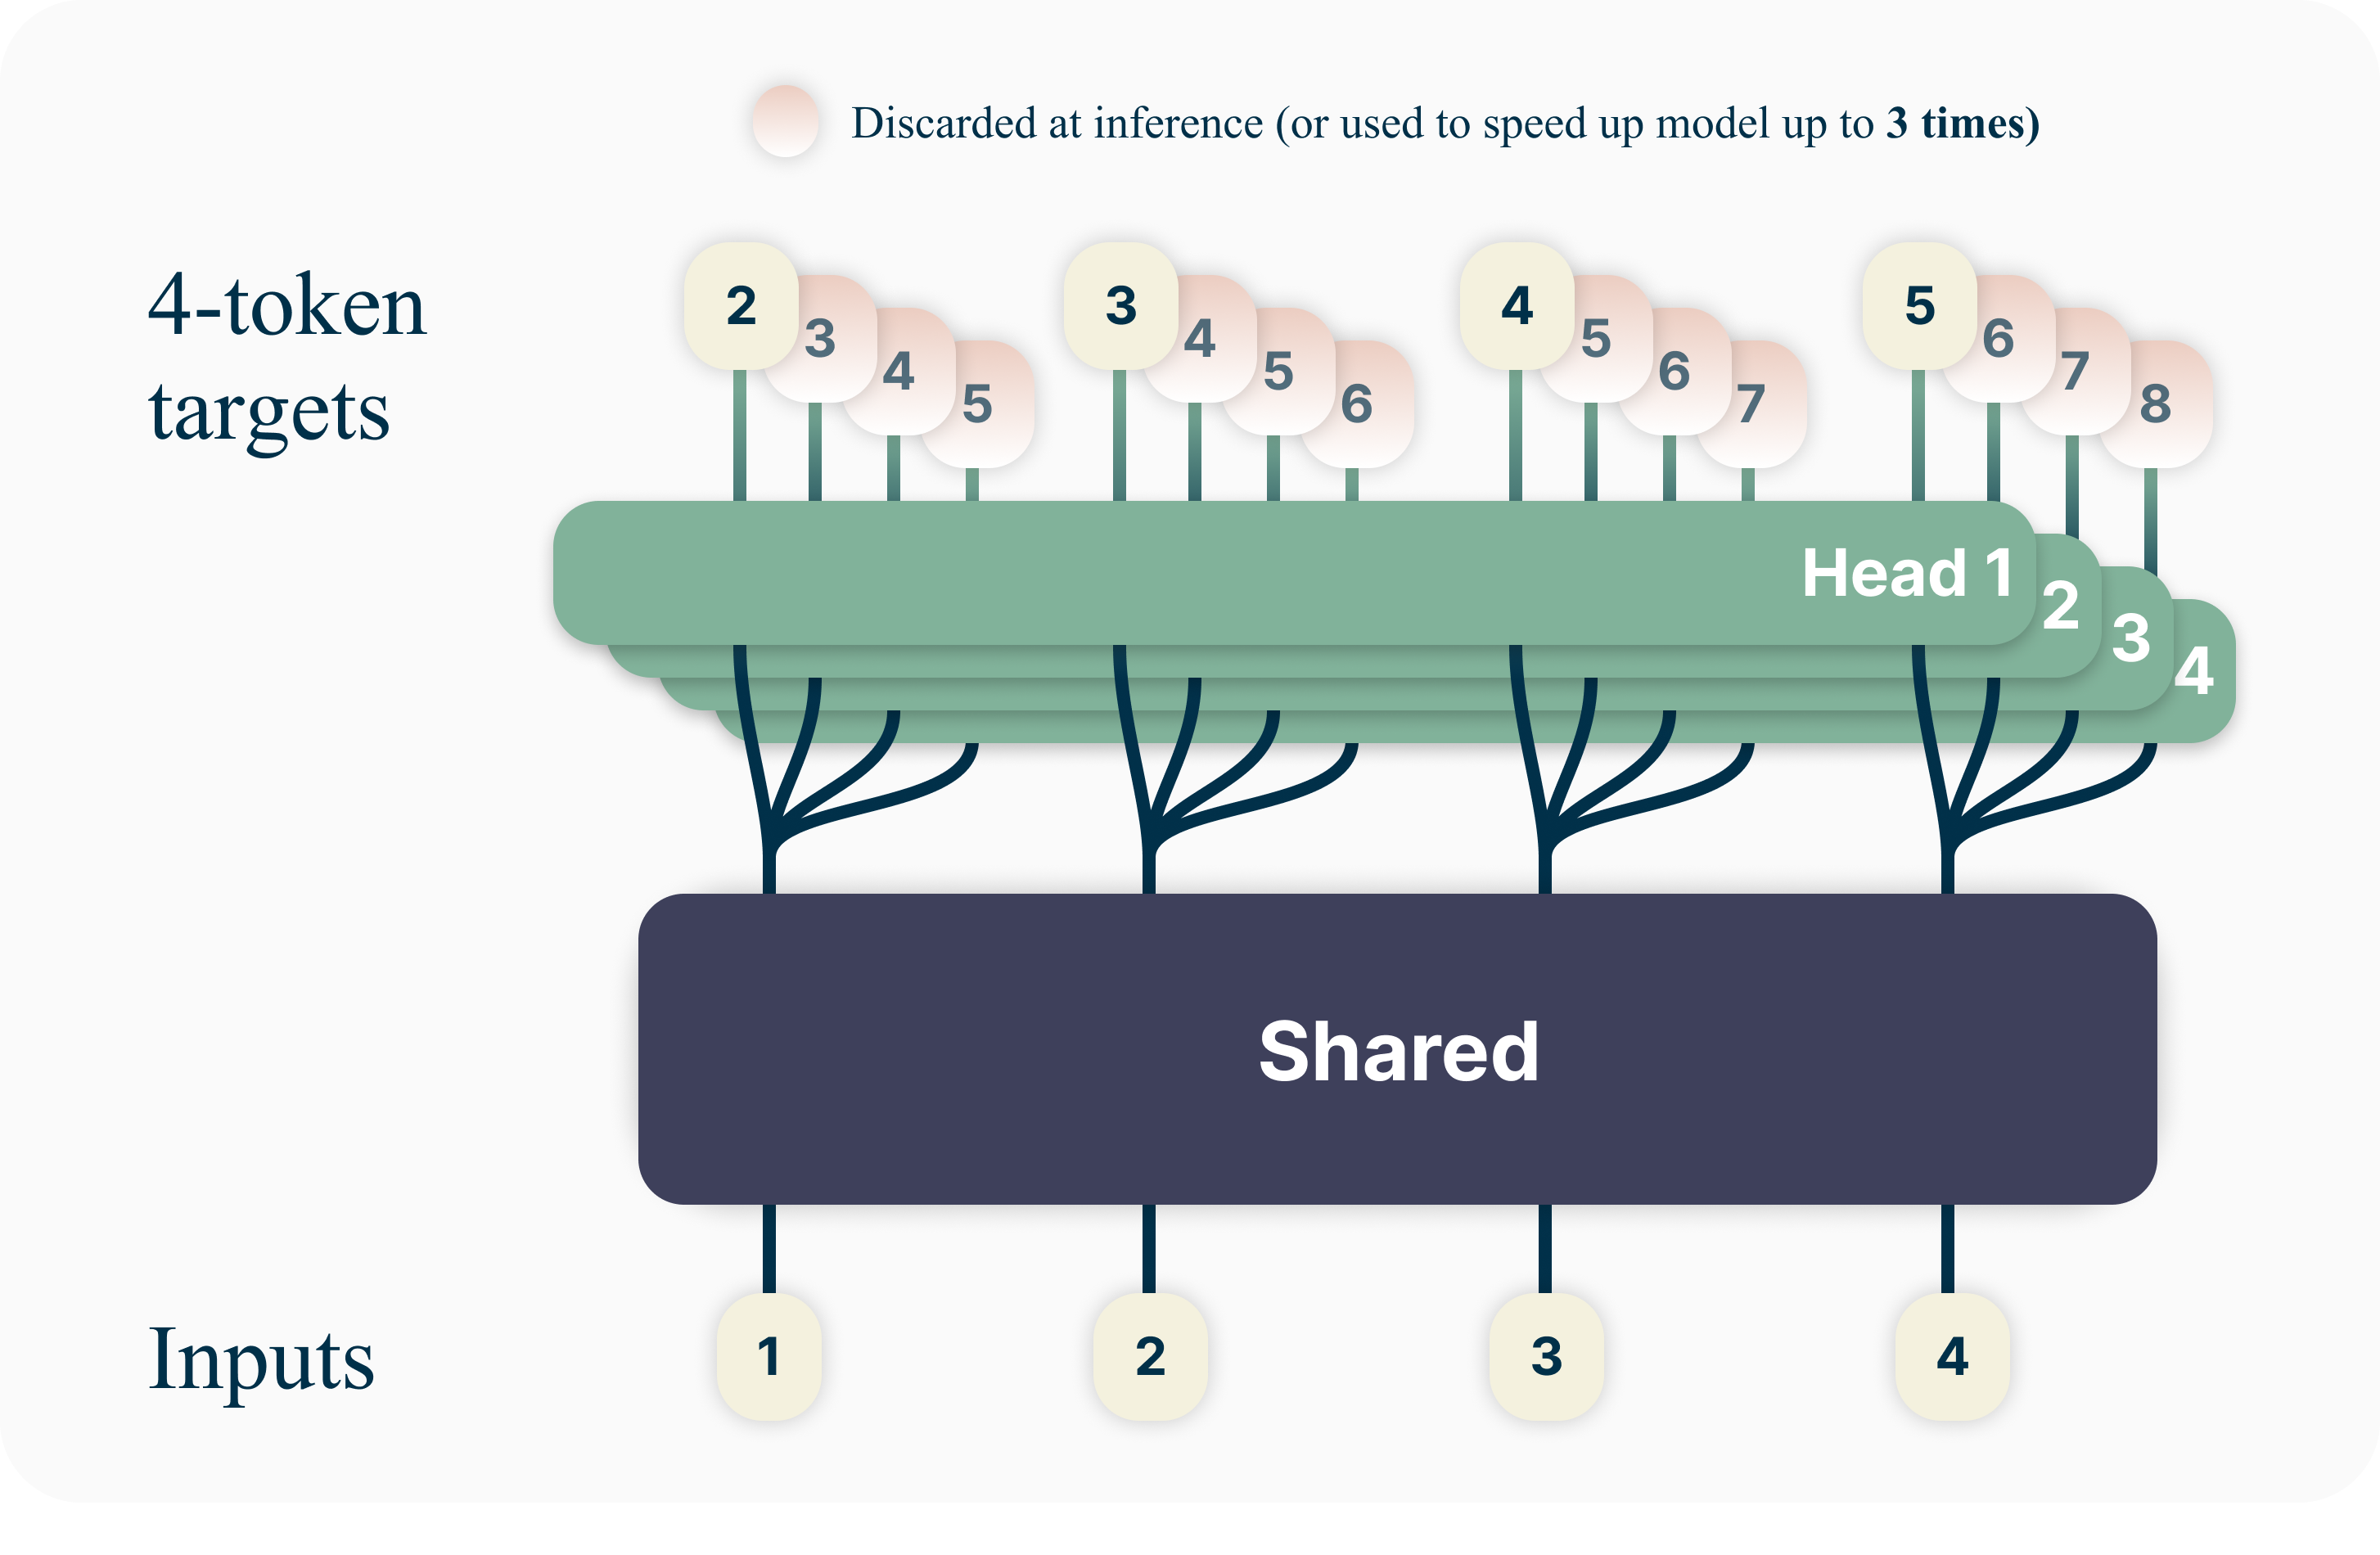
\includegraphics[width=\linewidth,height=0.55\textheight,keepaspectratio]{images/research-frontiers/mtp_fig1_architecture.png}
    \end{columns}
    \vspace{0.2em}
    \src{Gloeckle et al., ``Better \& Faster Large Language Models via Multi-token Prediction,'' \href{https://arxiv.org/abs/2404.19737}{arXiv:2404.19737}, Figure 1. DeepSeek-AI, \href{https://arxiv.org/abs/2412.19437}{arXiv:2412.19437}. Red Hat Developer, FastMTP article (Sep 2026).}
\end{frame}

\begin{frame}{2026: Drafters That Do Not Autoregress}
    \begin{columns}[T,onlytextwidth]
        \column{0.64\textwidth}
        \begin{itemize}\itemsep0.45em
            \item \textbf{DFlash (ICML 2026).} A small \emph{block-diffusion} drafter writes a whole block in one pass, conditioned on the target's hidden features. Lossless, over 6x, up to 2.5 times EAGLE-3's speedup.
            \item \textbf{Saguaro.} While the target verifies, a drafter on separate hardware already drafts for the likely outcomes. About 30\% faster than tuned speculative decoding.
            \item \textbf{Gemma 4} ships a 4-layer drafter that reads the main model's KV cache. Its output layer picks among 4,096 token clusters, not 262,000 tokens.
        \end{itemize}
        \column{0.34\textwidth}
        \centering
        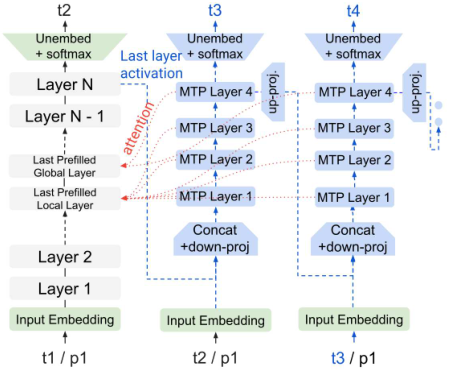
\includegraphics[width=\linewidth,height=0.5\textheight,keepaspectratio]{images/research-frontiers/gemma4_fig1_mtp_drafter.png}
    \end{columns}
    \vspace{0.2em}
    \caveat{NVIDIA reports up to 15x for DFlash on gpt-oss-120b. That is a vendor blog, on its newest hardware.}
    \src{Chen, Liang, Liu, ``DFlash,'' \href{https://arxiv.org/abs/2602.06036}{arXiv:2602.06036}. Kumar, Dao, May, ``Speculative Speculative Decoding,'' \href{https://arxiv.org/abs/2603.03251}{arXiv:2603.03251}. Gemma 4, \href{https://arxiv.org/abs/2607.02770}{arXiv:2607.02770}, Figure 1. NVIDIA developer blog (June 2026).}
\end{frame}

\subsection{Token Pruning and KV-Cache Compression}

\begin{frame}{Token Pruning: Three Places to Drop Tokens}
    \begin{center}
    \footnotesize
    \renewcommand{\arraystretch}{1.15}
    \begin{adjustbox}{max width=\linewidth}\begin{tabular}{>{\raggedright\arraybackslash}p{1.7cm}>{\raggedright\arraybackslash}p{2.0cm}>{\raggedright\arraybackslash}p{5.4cm}>{\raggedright\arraybackslash}p{3.1cm}}
        \toprule
        \textbf{Where} & \textbf{Method} & \textbf{Rule} & \textbf{Reported result} \\
        \midrule
        Prompt text & LLMLingua-2 & a small classifier keeps or drops each token & 2x to 5x shorter prompts \\
        KV cache & SnapKV & keep what the last 32 prompt tokens attend to & 8.2x less memory at 16K \\
        KV cache & PyramidKV & keep more in low layers, less in high ones & full quality with 12\% of the cache \\
        Attention & DeepSeek DSA & a trained indexer picks the top 2,048 keys & in production (Day 1) \\
        \bottomrule
    \end{tabular}\end{adjustbox}
    \end{center}
    \begin{itemize}\itemsep0.4em
        \item \textbf{The failure nobody tested at first.} SnapKV keeps what \emph{this} question needs. The next turn may need what was evicted. On SCBench, methods that drop KV entries struggle in multi-turn use.

        \item \textbf{Trend:} selection moved into training. DeepSeek-V4.1-Flash reports about 890 bytes of KV per token.
    \end{itemize}
    \src{Pan et al., \href{https://arxiv.org/abs/2403.12968}{arXiv:2403.12968}. Li et al., ``SnapKV,'' \href{https://arxiv.org/abs/2404.14469}{arXiv:2404.14469}. Cai et al., ``PyramidKV,'' \href{https://arxiv.org/abs/2406.02069}{arXiv:2406.02069}. Li, Jiang et al., ``SCBench,'' \href{https://arxiv.org/abs/2412.10319}{arXiv:2412.10319}. DeepSeek-AI, \href{https://arxiv.org/abs/2609.19969}{arXiv:2609.19969}.}
\end{frame}

\subsection{Compression Beyond Quantisation}

\begin{frame}{Pruning Weights: ``50\% Sparse'' Is Not ``2x Faster''}
    \begin{itemize}\itemsep0.3em
        \item \textbf{Wanda} needs no retraining. It scores each weight by its size \emph{times} the norm of the input it multiplies:
        $S_{ij} = \lvert W_{ij}\rvert \cdot \lVert X_j\rVert_2$.
    \end{itemize}
    \begin{center}
    \small
    \begin{adjustbox}{max width=\linewidth}\begin{tabular}{lcccc}
        \toprule
        \textbf{WikiText perplexity at 50\% sparsity} & \textbf{LLaMA-7B} & \textbf{13B} & \textbf{30B} & \textbf{65B} \\
        \midrule
        Magnitude pruning & 17.29 & 20.21 & 7.54 & 5.90 \\
        SparseGPT (minutes of solving) & 7.22 & 6.21 & 5.31 & 4.57 \\
        \rowcolor{KAUSTcyan!12} Wanda (seconds) & 7.26 & 6.15 & 5.24 & 4.57 \\
        \bottomrule
    \end{tabular}\end{adjustbox}
    \end{center}
    \begin{itemize}\itemsep0.35em
        \item \textbf{Does it run faster?} Unstructured zeros do not. The hardware-friendly 2:4 pattern gives about 1.6x on the matrix multiply alone.
        \item \textbf{End to end,} the first one-shot result on recent GPUs is \alert{1.2x} in decoding (SpenseGPT, 2026), and only by leaving some regions dense.
    \end{itemize}
    \src{Sun, Liu, Bair, Kolter, ``Wanda,'' \href{https://arxiv.org/abs/2306.11695}{arXiv:2306.11695}, Tables 3 to 5. Frantar, Alistarh, ``SparseGPT,'' \href{https://arxiv.org/abs/2301.00774}{arXiv:2301.00774}. Lee, Hwang, Rajbhandari, ``SpenseGPT,'' \href{https://arxiv.org/abs/2606.10445}{arXiv:2606.10445}.}
\end{frame}

\begin{frame}{Structured Pruning Ships When Distillation Follows It}
    \begin{itemize}\itemsep0.35em
        \item Removing whole neurons or layers gives an ordinary dense model that any runtime can serve.
        \item \textbf{Read the headline twice.} LLM-Pruner's ``keeps 94.97\% of performance'' is its best row (60.07 of 63.25). Layer removal keeps multiple-choice scores while summarisation nearly collapses.
    \end{itemize}
    \begin{center}
    \small
    \begin{adjustbox}{max width=\linewidth}\begin{tabular}{lccc}
        \toprule
        \textbf{Llama-3.1 8B to 4B (NVIDIA Minitron)} & \textbf{MMLU} & \textbf{Throughput} & \textbf{Training tokens} \\
        \midrule
        Original 8B & 0.6528 & 1.0x & 15T \\
        \rowcolor{KAUSTcyan!12} Width-pruned 4B & 0.6053 & about 1.8x & 94B \\
        Depth-pruned 4B & 0.5871 & about 2.7x & 94B \\
        \bottomrule
    \end{tabular}\end{adjustbox}
    \end{center}
    \begin{itemize}\itemsep0.35em
        \item \textbf{The recipe:} train the largest model once, prune by activation importance, retrain with distillation only. \textbf{Width keeps accuracy. Depth buys throughput.}
    \end{itemize}
    \src{Ma, Fang, Wang, ``LLM-Pruner,'' \href{https://arxiv.org/abs/2305.11627}{arXiv:2305.11627}, Table 1. Men et al., ``ShortGPT,'' \href{https://arxiv.org/abs/2403.03853}{arXiv:2403.03853}. Muralidharan et al., \href{https://arxiv.org/abs/2407.14679}{arXiv:2407.14679}. NVIDIA developer blog, Llama-3.1-Minitron 4B (Aug 2024).}
\end{frame}

\begin{frame}{Low-Rank Compression in One Equation}
    \begin{itemize}\itemsep0.3em
        \item Plain SVD of $W$ fails: a small singular value can still matter for the \emph{inputs the layer sees}.
        \item \textbf{SVD-LLM} whitens first. With $SS^\top = XX^\top$, decompose $WS = U\Sigma V^\top$ and truncate. Each dropped singular value then costs exactly its own size in output error:
        \[
            L = \lVert WX - W'X\rVert_F, \qquad L_i = \sigma_i
        \]
    \end{itemize}
    \begin{center}
    \small
    \begin{adjustbox}{max width=\linewidth}\begin{tabular}{lcccc}
        \toprule
        \textbf{LLaMA-7B, WikiText-2 perplexity} & \textbf{20\%} & \textbf{40\%} & \textbf{60\%} & \textbf{80\%} \\
        \midrule
        Plain SVD & 20,061 & 52,489 & 105,474 & 687,291 \\
        ASVD (activation-scaled) & 11.14 & 1,407 & 57,057 & 80,425 \\
        \rowcolor{KAUSTcyan!12} SVD-LLM & 7.73 & 9.27 & 15.00 & 31.79 \\
        \bottomrule
    \end{tabular}\end{adjustbox}
    \end{center}
    \begin{itemize}\itemsep0.3em
        \item \textbf{Reality check (2026):} one benchmark of five SVD methods finds end-to-end speedups \emph{``often limited''}. With custom kernels, FlashSVD reaches 1.44x on average.
    \end{itemize}
    \src{Wang, Zheng, Wan, Zhang, ``SVD-LLM,'' ICLR 2025, \href{https://arxiv.org/abs/2403.07378}{arXiv:2403.07378}, Theorem 3.2 and Table 1. Yuan et al., \href{https://arxiv.org/abs/2312.05821}{arXiv:2312.05821}. Shao et al., ``LowRankArena,'' \href{https://arxiv.org/abs/2608.26389}{arXiv:2608.26389}. Wu et al., \href{https://arxiv.org/abs/2605.08314}{arXiv:2605.08314}.}
\end{frame}

\begin{frame}{Efficiency: What to Remember}
    \begin{itemize}\itemsep0.55em
        \item Speculation moved \textbf{inside the model}: heads (Medusa), feature drafters (EAGLE-3), trained multi-token modules, block-diffusion drafters (DFlash).
        \item Its gains are real at batch size 1 and \textbf{shrink at high batch}. Always ask for the serving regime.
        \item Post-hoc KV eviction fails in \textbf{multi-turn} use. Production systems train the selection in.
        \item For pruning and low-rank methods, measured end-to-end gains are \textbf{1.2x to 1.5x}, far from the FLOP count.
        \item What ships is \textbf{prune, then distil}: a smaller dense model that needs no special kernel.
    \end{itemize}
    \vspace{0.4em}
    \takeaway{\textbf{Next.} DFlash drafts a whole block in parallel with diffusion, then lets an autoregressive model check it. What if the diffusion model \emph{is} the language model?}
\end{frame}
